\documentclass{article}

% \usepackage{corl_2018}
\usepackage[final]{corl_2018} % Uncomment for the camera-ready ``final'' version
\usepackage{wrapfig}

\usepackage{subcaption}
\usepackage{graphicx}

\usepackage{amsmath}
\usepackage{amsfonts}
\usepackage{mathtools}

\providecommand\todo[1]{\textcolor{Red}{#1}}

\usepackage[utf8]{inputenc} % allow utf-8 input
\usepackage[T1]{fontenc}    % use 8-bit T1 fonts
\usepackage{hyperref}       % hyperlinks
\usepackage{url}            % simple URL typesetting
\usepackage{booktabs}       % professional-quality tables
\usepackage{amsfonts}       % blackboard math symbols
\usepackage{nicefrac}       % compact symbols for 1/2, etc.
\usepackage{microtype}      % microtypography
\usepackage[svgnames]{xcolor}
\usepackage{authblk}

\providecommand\comment[1]{\textbf{COMMENT:} \textcolor{Magenta}{#1}}

\setlength{\bibsep}{4pt plus 0.3ex}

% \title{Precision via Persistence: Closed-Loop Robotic Manipulation with Self-Supervised Learning}
\title{Robustness via Retrying: Closed-Loop Robotic Manipulation with Self-Supervised Learning}
% How about this title? We're actually getting more robustness than precision from the tracking..
% Hmm. Maybe Robustness via Retrying? Though, I like Persistence.

%%SL.06.12: I really like the title! Especially the first part. I do not think it's regrettable though that it doesn't really say much about how the method works, but maybe that's OK? It's definitely very catchy and manages to capture the main *new* contribution quite well. Maybe you can work in the word "visual" or "vision-based" before closed-loop? that makes it much more impressive -- lots of things are closed-loop, but not many things close the loop on vision
%%CF.06.11: How about the following: Precision via Persistence: Closed-Loop Robotic Manipulation with Self-Supervised Learning
%%SL.04.20: Let's think about the title a bit more. This seems like a reasonable starting point. But first let's list the main ideas that seem to make the work exciting:
%The ability to fix mistakes
%The ability to reach goal images by comparing them directly to the current image
%The ability to achieve goals to high accuracy
%The ability to do on-policy data collection to acquire more complex skills like grasping
% Some things are exciting, but not inherently new to this work, including: self-supervised, closed-loop, etc.
%  on the other hand, instead of the somewhat generic 'self-supervised learning,' we can probably come up with something
%  a bit more descriptive: one thing that makes our approach different is that, with on-policy data collection, the robot
%  is essentially setting its own goals and then attempting to reach them, so we can call it something like 'self-directed play'
% Some things are exciting but not mentioned, including the fact that this is done with raw images...
% Here are a few thoughts I have about possible titles:
%Visual Learning with Self-Directed Play: Acquisition of Complex Robotic Skills with Direct Video Prediction
%Self-Directed Play with Visual Recall: Learning Manipulation Tasks by Reaching Previous Observations
%Learning Vision-Based Robotic Skills with Self-Directed Play
%...
% Another direction we could go is to emphasize that the method can succeed even with an imperfect predictor, by trying again, but I'm not really sure how to fit that into a very concise title
%%SL.04.20: it would also be good to get some illustrated diagram put together soon to explain how the method works... I feel like a diagram might be quite important here

% The \author macro works with any number of authors. There are two
% commands used to separate the names and addresses of multiple
% authors: \And and \AND.
%
% Using \And between authors leaves it to LaTeX to determine where to
% break the lines. Using \AND forces a line break at that point. So,
% if LaTeX puts 3 of 4 authors names on the first line, and the last
% on the second line, try using \AND instead of \And before the third
% author name.

% NOTE: authors will be visible only in the camera-ready (ie, when using the option 'final'). 
% 	For the initial submission the authors will be anonymized.

% \author{
%   David S.~Hippocampus\\
%   Department of Electrical Engineering and Computer Sciences\\
%   University of California Berkeley 
%   United States\\
%   \texttt{hippo@berkeley.edu} \\
%   %% examples of more authors
%   %% \And
%   %% Coauthor \\
%   %% Affiliation \\
%   %% Address \\
%   %% \texttt{email} \\
%   %% \AND
%   %% Coauthor \\
%   %% Affiliation \\
%   %% Address \\
%   %% \texttt{email} \\
%   %% \And
%   %% Coauthor \\
%   %% Affiliation \\
%   %% Address \\
%   %% \texttt{email} \\
%   %% \And
%   %% Coauthor \\
%   %% Affiliation \\
%   %% Address \\
%   %% \texttt{email} \\
% }


\author[1]{Frederik Ebert}
\author[1]{Sudeep Dasari}
\author[1]{Chelsea Finn}
\author[1]{Alex X. Lee}
\author[1]{Sergey Levine}

\affil[1]{\footnotesize Department of Electrical Engineering and Computer Sciences, UC Berkeley, United States}

\affil[ ]{\texttt{\{febert, sdasari, cbfinn,alexlee\_gk,svlevine\}@berkeley.edu}}

\begin{document}
% \nipsfinalcopy is no longer used

\maketitle

\begin{abstract}
% Understanding how the world works -- which actions lead to which future events -- can allow humans to act intelligently in complex and unfamiliar situations. Crucially, understanding and predicting physical interactions does not require any supervision beyond observation of one's own actions and their consequences. This makes
Prediction is an appealing objective for self-supervised learning of behavioral skills in particular for autonomous robots. However, incorporating prediction of future sensory inputs into an end-to-end framework for decision making and control poses a number of major challenges. How should the predictive model be used? What happens when the predictions are inaccurate? In this paper, we tackle these questions by proposing a method for learning complex robotic skills from raw image observations, using only autonomously collected experience. We show that even an imperfect model can complete complex tasks if it can continuously retry, but this requires the model to not lose track of the objective (e.g., the object of interest). By incorporating  learned registration into our method, we can enable a robot to continuously retry the task until it gets it right. We demonstrate that this idea can be combined with a video-prediction based controller to enable complex behaviors to be learned from scratch using only raw visual inputs, including grasping, repositioning objects, and non-prehensile manipulation. Our real-world experiments demonstrate a model trained with 160 robot hours of autonomously collected data is able to successfully master complex manipulation tasks with a wide range of objects not seen during training. 

\end{abstract}
%%SL.04.20: Here is my attempt at an alternative abstract that I think brings out some of the more exciting things about the work. Maybe this can serve as some inspiration for how to get a more focused abstract in place that at the same time still touches on the big picture stuff:
%Understanding how the world works -- which actions lead to which future events -- can allow humans and animals to act intelligently in complex and unfamiliar situations. Crucially, understanding and predicting physical interactions does not require any supervision beyond observation of one's own actions and their consequences. This makes prediction an appealing objective for self-supervised learning of behavioral skills, for example for autonomous robots. However, incorporating prediction of future sensory inputs into an end-to-end framework for decision making and control poses a number of major challenges. How should the data for learning to predict be collected? How should the predictive model be used? What happens when the predictions are inaccurate? In this paper, we tackle these questions by proposing a method for learning complex robotic skills from raw image observations, using only autonomously collected experience. Our method is based on two key ideas. First, we use self-directed play to collect data, where the robot autonomously proposes goals and then attempts to execute them. We demonstrate in simulation that this substantially improves performance over random data collection. Second, we observe that even an imperfect model can complete complex tasks if it can continuously retry, but this requires the model to not lose track of the objective (e.g., the object of interest). By incorporating end-to-end learned registration into our method, we can enable the robot to continuously retry the task until it gets it right. We demonstrate that these two ideas can be combined to enable complex behaviors to be learned from scratch using only raw visual inputs, including grasping and repositioning objects, non-prehensile pushing, and maneuvering objects around obstacles. Our real-world experiments demonstrate a model trained with ??? hours of autonomously collected experience with self-directed play, and testing on previously unseen objects.

\section{Introduction}

\begin{wrapfigure}{r}{.4\columnwidth}
\vspace{-5mm}
\centering
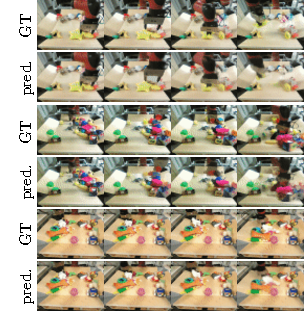
\includegraphics[width=0.4\columnwidth,trim={3.2mm 0 0 0},clip]{images/video_prediction}
\caption{\small{Ground truth and predictions from the model (only every 4 frames are shown). These examples show grasping, pushing, and simultaneous grasping and dragging. \todo{consider replacing with sudeep diagram?}}}
\label{fig:video_prediction}
\vspace{-0.2in}
\end{wrapfigure}

Humans have the ability to learn complex skills such as manipulating objects through millions of interactions with their environment during their lifetime.
These interactions enable us to acquire a general understanding of the physical world and, notably, do not require significant supervision beyond observation of one's own actions and their consequences. Hence, self-supervised learning through prediction is an appealing direction of research as it enables intelligent systems to leverage and learn from massive amounts of unlabeled raw data to autonomously acquire general skills. Yet, self-supervised learning systems using predictive models of sensory inputs present a number of challenges: planning needs to account for imperfections in the predictive model and the robot needs a grounded mechanism for evaluating predicted futures.
How can we enable systems to plan to perform complex tasks from raw sensory observations, even when the predictions are not always accurate?

Prior work on self-supervised robot learning has enabled robots to learn rudimentary, short-term manipulation skills such as grasping~\cite{lerrel,google_handeye}, singulation~\cite{princeton_pushgrasp}, pushing~\cite{foresight,sna}, poking~\cite{pulkit}, and other arm motions~\cite{se3_control}. The question that we are concerned with in this work is: can self-supervised predictive models of raw visual observations be used to perform more complex and realistic tasks, especially tasks that are temporally extended? 
%, closed-loop control of multiple forms of behavior and goals through self-supervision remains an open problem.
%Prior work has demonstrated that video prediction can be used for rudimentary, short-term robotic manipulation tasks in the real world, such as pushing objects~\cite{}. The question we are concerned with in this work is: can direct video prediction be used to perform more complex and realistic tasks, especially tasks that are temporally extended? 
While this might seem exceedingly challenging due to the difficulty of long-term prediction of images, we make use of the well-known principle of model-predictive control (MPC) that allows targeting long-terms goals with a relatively short prediction horizons. To allow effective replanning, we need a planning objective that allows the robot to reliably make progress towards the goal.
%that is optimized by a short-horizon planner allowing to reliably make progress towards the goal. 

%While this might seem exceedingly challenging due to the difficulty of long-term prediction of images, we make the following observation: that make it feasible to perform relatively long-horizon tasks. First, we observe that short-horizon planning can still give us a good indication of the potential for a plan to achieve a long-term goal, if provided with the right cost function. This fact has been known for decades, and is the basis for model-predictive control: iterative short-horizon replanning that aims to achieve long-term goals. Yet, maintaining an accurate estimate of the cost function throughout planning is crucial.
We propose a cost function based on image-to-image registration, which we demonstrate can itself be learned without any human supervision using the same exact dataset as the one used to train the predictive model. The key element that enables our method to perform long-horizon tasks is that, using our cost function, the robot can always evaluate the distance to the goal, allowing it to continuously retry, so that even flawed predictions allow for an eventual successful execution. 



%Closed-loop control allows the robot to be persistent, correcting for mistakes caused by inevitable model inaccuracies and continuously retrying until it succeeds.
%Further, learning models that can be used to plan multiple types of behaviors is critical for learning general-purpose control.
%%SL.06.12: there are two ideas above: (1) learning models that can be used for various tasks is important for general-purpose control (2) retrying is a good idea; these ideas are kind of stuck together awkwardly a bit, can we push them apart so that one builds on the other?
%In this work, we aim to develop a learning system that interacts with the environment autonomously, building a model that can be used to plan a variety of motions, including pushing, grasping, and placing, while enabling the agent to continuously try and retry the task until it succeeds.
%%SL.06.12: the title says something about being precise -- where does that come in?

%A robot equipped with action-conditioned predictive models of future observations has some understanding of the physical world and how it changes as a consequence of its actions. Such model could then be used by the robot to plan multiple types of behaviors for general-purpose control. These models can be learned through self-supervision, whereby the robot interacts with the environment through random actions while observing through its sensors. In our work, we use a video prediction model that predicts future frames conditioned on actions and past frames.

%%AL.06.13: I think we need two paragraphs that contains the following information:
% Paragraph on self-supervised learning. Massive amounts of self-supervised data. Action-conditioned video prediction model that predicts future frames by implicitly transforming pixels from previous frames via image-space flow fields. These flows can be used for planning given a designated pixel position in the first frame and goal pixel position in the goal frame (say how it's done). Forward models can deviate from the truth very quickly due to compounding errors. Naturally, replanning (MPC). However, we don't have good cost functions since we have lost designed pixel position in the new first frame. Solution?
% Paragraph on registration. Track designed pixel position. Allows for more precise retrying. Registration registers to both first and goal frames, so can be accurate near beginning and end of trajectory.


%%SL.04.20: I would recommend reading through this carefully and noting the key points that we need to touch on in an introduction: https://cs.stanford.edu/people/widom/paper-writing.html


We demonstrate our method on the task of maneuvering unknown objects in a table-top setting using a robot manipulator. To autonomously learn to perform manipulation skills with high-fidelity, tasks need to be specified in way that allows for precision and retrying. We specify a goal by providing an image of the desired configuration along with user-annotated positions of the objects of interest\footnote{This also allows the user to specify distractor objects that can be ignored in the goal image}. This provides a straight-forward and grounded mechanism for a human to provide a goal in the observation space of the robot.
Building upon prior methods that use self-supervised predictive models for control~\cite{foresight,sna,se3_control}, we develop a method that can plan actions with a video prediction model to achieve the desired state specified in the goal image.
%%SL.06.12: I feel like maybe we should explicitly say that our method builds on prior work (foresight, sna), since in this case the contribution might actually be easier to understand if we explicitly frame it in terms of prior work. It might open us up to accusations that the work is incremental, but I think that is less bad than a lack of clarity about the nature of the contribution

The main contribution of this work is a method for computing the planning cost based on image-to-image registration by using a learned registration model to find correspondences  between the current image and both the goal image and the initial image.
%We train a deep convolutional network to find these correspondences by learning an image-to-image warping function in a self-supervised manner. 
This allows closed-loop control, enabling the robot to persistently attempt the task until completion. In contrast to the short-horizon pushing skills and arm motions demonstrated in prior work~\cite{foresight,sna,se3_control}, we show that our video prediction model can be used to perform longer-term manipulations, autonomously choosing when to push or to  pick objects, and, when provided enough time, accomplish tasks significantly more consistently.
In addition we show that a joint pushing and grasping-policy can be emerge from pure self-supervised learning. Furthermore by using with two separate views for video-prediction and task specification, 3D-tasks manipulation tasks can be solved.

%Compared to prior work on self-supervised learning and hand-engineered tracking modules, we find that our approach is able to perform a variety of object manipulation tasks and, when provided enough time, achieve tasks significantly more consistently.

%%SL.06.12: Some high level comments on the introduction: Currently, it doesn't really talk about grasping -- it just abstractly says that there are multiple skills, but not what those skills are. Can we elaborate on this point a little bit? I think the current intro is definitely better, but we should try to do a better job of coming up with the story. I think we should make sure we touch on the following points/questions:
%Prior work has demonstrated that video prediction can be used for rudimentary, short-term robotic manipulation tasks in the real world, such as pushing objects~\cite{}. The question we are concerned with in this work is: can direct video prediction be used to perform more complex and realistic tasks, especially tasks that are temporally extended? While this might seem exceedingly challenging due to the difficulty of long-term prediction of images, we make the following observations that make it feasible to perform relatively long-horizon tasks. First, we observe that short-horizon planning can still give us a good indication of the potential for a plan to achieve a long-term goal, if provided with the right cost function. This fact has been known for decades, and is the basis for model-predictive control: iterative short-horizon replanning that aims to achieve long-term goals. For video prediction, we propose a cost function based on image registration, which we demonstrate can itself be learned without any human supervision using the same exact dataset as the one used to train the predictive model. The second idea that enables our method to perform long-horizon tasks is that, if the robot can always evaluate the goal, it can continuously retry, so that even flawed predictions allow for an eventual successful execution. We use the same learned registration model to enable this retrying behavior.
%
%In contrast to the short-horizon pushing skills demonstrated in prior work~\cite{}, we show that our video prediction model can be used to perform longer-term manipulations and automatically choose to push and pick objects, acquiring rudimentary grasping behaviors entirely via video prediction.

%this registration network learns a function that transforms images from arbitrary timesteps along a video to match frames from other timesteps. 









\vspace{-0.1cm}
\section{Related Work}
\vspace{-0.1cm}

Prior work has studied pushing with hand-engineered models or features \cite{hermans2013learning,salganicoff1993vision}, as well as 

In prior work \cite{hermans2013learning,salganicoff1993vision}, pushing of unknown objects is learned from interaction data between the robot and objects. However the models employed there rely on hand-engineered input features which can make it hard to scale to complex real-world scenarios. 
It as been shown in \cite{goldfeder2009data} and others that grasps on unseen objects can be found by matching the sensed 3D geometry to a database of precomputed object-grasp pairs, which has the downside that physical properties such as mass and friction are ignored. Furthermore most prior approaches are not capable of selecting whether a grasping, pushing or dragging strategy is better suited to solve the given task and also do not exhibit a "retrying" behavior for recovering from failure.
Video-prediction based manipulation is more general than many existing methods for robotic manipulation such as grasping specific \cite{lenz2015deep, goldfeder2009data, zeng2017robotic} or pushing specific works \cite{hermans2013learning, salganicoff1993vision} because it does not require any human intervention at training time, since it is fully self-supervised. Also it does not make any assumptions about the dimensionality of the state space.

Many self-supervised robot learning methods have focused on predicting the outcome of a particular event such as grasp success~\cite{lerrel,google_handeye,princeton_pushgrasp} or crashing~\cite{crashing,greg_kahn_uncertainty}. Consequently, these approaches can only recover a single policy that optimizes the probability of the predicted event. Instead, we aim to acquire a model that can be reused for multiple goals and behaviors. To do so, we build upon prior works that learn to predict the sequence of future observations, which can be used to optimize with respect to a variety of goals~\cite{foresight,sna,se3_control}. Unlike~\cite{se3_control}, we demonstrate complex object manipulations with previously-unseen objects from RGB video. In contrast to prior self-supervised visual planning works~\cite{foresight,sna}, we can perform substantially longer tasks, by using image registration with respect to a goal image.

Goal observations have been previously used for specifying a reward function for robot learning systems~\cite{jagersand1995visual,deguchi1999image,e2c,dsae}. Unlike these methods, we use a learned registration to the goal image for measuring distance to the goal rather than distance in a learned feature space. Distances in unconstrained feature spaces can be arbitrary, while registration inherently measures how pixels should move and can therefore provide a calibrated distance metric with respect to the goal. 

A related problem is visual servoing, where visual feedback is used to reach a goal configuration~\cite{hutchinson1996tutorial,kragic2002survey,desouza2002survey}.
Traditional approaches aim to minimize distances of feature points~\cite{feddema1989vision,espiau1992servo,wilson1996relative}, or pixel intensities~\cite{caron2013photometric}. Learning and convolutional networks have also been incorporated into visual servoing~\cite{saxena2017servoing,bateux2018servoing,lee2017servoing,google_handeye}. Unlike servoing approaches that use reactive control laws, we use multi-step predictive models to achieve temporally extended goals, while still using continuous visual feedback for retrying at every step. Further, our method performs non-prehensile manipulation, while visual servoing typically assumes fully actuated control, often with a known Jacobian.

Model-predictive control (MPC)~\cite{camacho2013model} has proven successful in a variety of robotic tasks~\cite{shim2003decentralized,allibert2010predictive,howard2010receding,williams2017information,deep_mpc}.
MPC involves planning with a short horizon and re-planning as the execution progresses, providing the foundation of persistent retrying and the ability to overcome inaccuracies in the predictive model. However, as we later show, maintaining an accurate model of the \emph{cost} used for planning throughout an episode is critical, and has prevented prior work on visual foresight~\cite{foresight,sna} from moving beyond short-term tasks.
Our primary contributions is a grounded mechanism for evaluating the planning cost of visual predictions, allowing persistent re-planning with video prediction models.

It possible to use off-the-shelf trackers~\cite{lucas1981iterative,brox2004high,babenko2009visual,mei2009robust} to help address this issue. However, these trackers usually only have a limited capability to adapt to the domain they are applied to, and can lose track during occlusions. A key advantage of our learned registration approach, inspired by \cite{meister2017unflow}, is that we can obtain registration success metrics for every point in the image and every pair of images and therefore we can propose a weighting scheme for the planning costs according to the \emph{uncertainty} of the individual registrations. Furthermore, since our method is completely self-supervised, it continues to improve as more data is collected by the robot.


\vspace{-0.1cm}
\section{Preliminaries}
\label{sec:prelim}
\vspace{-0.2cm}

Our visual MPC problem formulation follows the problem statement outlined in prior work~\cite{foresight}. In this setting, an action-conditioned video prediction model $g$, typically represented by a deep neural network, is used to predict future camera observations $\hat{I}_{1:T} \in \mathbb{R}^{T \times H\times W \times 3}$, conditioned on a sequence of candidate actions $a_{1:T}$, where the prediction horizon is $T$. This can be written as $\hat{I}_{1:T} = g(a_{1:T}, I_0)$, where $I_0$ is the frame from the current time-step. An optimization-based planner is  used to select the action sequence that results in an outcome that accomplishes a user-specified goal. This type of vision-based control is highly general, since it reasons over raw pixel observations without the requirement for a fixed-size state space, and has been demonstrated to generalize effectively to non-prehensile manipulation of previously unseen objects~\cite{foresight,sna}.

Visual MPC assumes the task can be defined in terms of pixel motion. In the initial image $I_0$ we define $n$ source pixel locations denoted by the coordinates $d_{0,i} \in \mathbb{N}^2$ (for $i \in [0,..n]$) and the analogous for the goal image $I_g$ denoted by $d_{g,i} \in \mathbb{N}^2$. Given a goal, visual MPC plans for a sequence of actions $a_{1:T}$
to move the pixel at $d_{0,i}$ to $d_{g,i}$. If this pixel lies on top of an object, this corresponds to moving that entire object to a goal position. Note that this problem formulation resembles visual servoing, but it is considerably more complex, since moving the object at $d_0$ might require complex non-prehensile or prehensile manipulation and long-horizon reasoning.
The planning problem is formulated as the minimization of a cost function $c$, which in accordance with prior work \cite{sna}, measures the distance between the predicted pixel positions $\hat{d}_{\tau}$ and the goal position $d_g$ for each pixel $i$:
\begin{align}
c = \sum^n_{i = 1}  \lambda_i c_i && c_i = \sum_{\tau = 1, \dots, T} \mathbb{E}_{\hat{d}_{\tau,i} \sim P_{\tau,i}} \left[\|\hat{d}_{\tau,i} - d_{g,i}\|_2\right]  
\label{eq:cost}
\end{align}
where $c_i\in \mathbb{R}$ are the costs per source pixel, $\lambda_i$ are weighting factors discussed in section \ref{sec:reg} and $P_{\tau,i}$ is the distribution over predicted pixel positions. The advantage of distance-based cost functions is that they are well-shaped and can be optimized efficiently. 

In this paper we use the video prediction model architecture developed by~\cite{savp}, where future images are generated by transforming past images. Starting with a distribution over initial positions of the designated pixel \mbox{$P_{t_0,i}\in\mathbb{R}^{H\times W}, \sum_{H,W} P_{t_0,i} = 1$} at time $t = 0$, the model predicts distributions over its positions $P_{t,i}$ at time $t \in \{ 1, \dots, T \}$ by exploiting the image transformations used to generate future frames. Planning is performed by sampling candidate actions sequences and optimizing using the cross-entropy method (CEM) \cite{cem-rk-13} to achieve the lowest possible cost $c$.

To obtain the best results with imperfect models, the action sequence is replanned at each real-world time step\footnote{We refer to timesteps in the real world as $t$ and to predicted time-steps as $\tau$.} $t \in \{0,...,t_{max}\}$ following the framework of model-predictive control (MPC): at each real-world step $t$, the first action of the best action sequence is executed. 
At the first real-world time step $t=0$, the distribution $P_{\tau=0,i}$ is initialized as 1 at the location of the designated pixel and zero elsewhere. In prior work \cite{sna, foresight}, in subsequent steps ($t > 0$),  the prediction of the previous step is used to initialize $P_{\tau=0,i}$. However this causes accumulating errors, often preventing the model from solving long-term tasks or responding to situations where the outcome of an action was different than expected. In effect, the model loses track of which object was designated in the initial image.









\vspace{-0.1cm}
\section{Retrying by Registration}
\label{sec:reg}
\vspace{-0.2cm}



%%SL.06.12: I think at least part of the motivation (maybe here or in the previous section) should include some discussion of how, in MPC, we can solve longer-horizon tasks by having a reasonable cost function that causes even a short-horizon planner to make steady progress toward the goal. From here, we can motivate that simply trying to match the image pixels of the target image is not a good cost, and part of the issue with long-horizon tasks via video prediction is really in the cost function. Prior work {ours} addresses this by using the motion predicted by the model to estimate positions of designated pixels (i.e., points on an object of interest) and measure their distance to the destination. But this requires tracking the object, and it's easy to lose track of the object during a complex manipulation where it might become occluded. In this work, we instead aim to estimate distances between images, registering the current image to the goal and using this registration to evaluate a distance. We will demonstrate in Section~\ref{something} that this substantially improves the performance of control via video-prediction, particularly on temporally extended tasks.

%Motivation for registering pixels
While self-supervision enables training powerful models to predict raw sensor inputs (among other quantities), using these model for control (e.g., with model-predictive control) poses the challenge of defining an appropriate cost function. One na\"{i}ve approach of formulating a cost function for video-prediction based control could be using the pixel-wise error between a \emph{goal image} and the predicted image. Goal images have the advantage that they are very general and do not make any domain specific assumptions. Minimizing this pixel-difference cost with respect to the action sequence passed into the model should result in a controller that tries to bring the system into the goal state. However there are a number of issues with this approach: first when objects in the image are far from the position in the goal image (e.g., they do not overlap) there is no gradient signal of the pixel-difference cost with respect to the actions. Second, due to the blurry predictions obtained from video-prediction model, the pixel-wise difference between the predictions and the goal image can become meaningless. Another possible approach would be to perform a registration between predicted video frames and the goal-image and using the average length of the warping vectors as a cost function for ``closeness" to the goal image; however, registering blurry prediction to a sharp goal-image poses a similar challenge as before. 

The main contribution of this work is a method for computing the planning cost based on image-to-image registration, which yields distances between tracked object and target location. As a result, the cost is well-shaped, allowing for efficient optimization.

\begin{wrapfigure}{r}{.5\columnwidth}
\vspace{-0.25in}
\centering
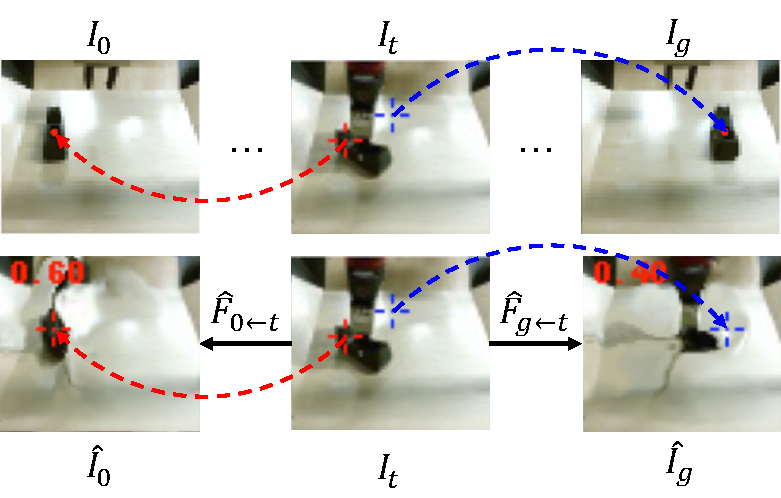
\includegraphics[width=0.5\columnwidth]{images/registration_singletime.pdf}
% \vspace{-0.1in}
\caption{\small{Closed loop control is achieved by registering the current image $I_t$ globally to the first frame $I_0$ and the goal image $I_g$. In this example registration to $I_0$ succeeds while registration to $I_g$ fails since the object in $I_g$ is too far away.}
\label{fig:reg_single}
\vspace{-0.2in}
}
\end{wrapfigure}


%%CF.06.15: the transition from the above to the below is rather abrupt.
\paragraph{Closed-loop video-prediction based control}

When the robot interacts with an object, the position of that object may change in unexpected ways, and therefore it is crucial that the system can update its belief of where the target object is. Prior work on visual MPC lacked this capability. To enable the agent to ``keep retrying" indefinitely until the task is accomplished we propose to use an image-to-image registration approach to find the target object in the current frame. 
We show that this tracking capability can be learned completely unsupervised from the data collected by the robot autonomously. As one might expect the self-supervised tracking approach works better for images that are closer to each other and sometimes fails when the entities in the image are too far apart. To increase accuracy and robustness in addition to the starting image our method can register to a goal-image. The goal image is optional and can be provided by a human or through demonstration.

\subsection{Test time procedure}

We will first describe the architecture at test time (see Figure~\ref{fig:registration_arch}). The start and goal images $I_0$ and $I_g$ are passed into the registration network $R$ which is trained to return flow maps $\hat{F}_{0 \leftarrow t} \in \mathbb{R}^{H \times W \times 2}$. The flow map is a vector field in $\mathbb{R}^2$ which describes the relative motion for every pixel between two frames.
\begin{align}
    \hat{F}_{0 \leftarrow t} = R(I_t, I_0) &&
    \hat{F}_{g \leftarrow t} = R(I_t, I_g)
\end{align}

The flow map $\hat{F}_{0 \leftarrow t}$ can be used to warp the image of the current time step $t$ to the start image $I_0$, and $\hat{F}_{g \leftarrow t}$ can be used to warp from $I_t$ to $I_g$ (see Figure \ref{fig:reg_single} for an illustration):
\begin{align}
    \hat{I}_0 = \hat{F}_{0 \leftarrow t} \diamond  I_t &&
    \hat{I}_g = \hat{F}_{g \leftarrow t} \diamond  I_t 
\end{align}
Where $\diamond$ denotes a bilinear interpolation operator which interpolates the pixel value bilinearly with respect to a location $(x,y)$ and its four neighbouring pixels in the image.
In addition to start and goal images, the user needs to specify one or several designated pixel positions (for simplicity showing only the case for one designated pixel) $d_0 \in \mathbb{N}^2$ in the start image and the corresponding pixels locations $d_g \in \mathbb{N}^2$ in the goal image (the goal image is optional) to define the task. While the registration network is trained to perform a global registration between the images, we only evaluate it at the points $d_0$ and $d_g$ chosen by the user. This results in a cost function that ignores distractors. For a current image $I_t$, $\hat{F}_{0 \leftarrow t}$ puts it in correspondence with $I_0$, and $\hat{F}_{g \leftarrow t}$ puts it in correspondence with $I_g$. The registration network is then used to find the pixel locations corresponding to $d_0$ and $d_g$ in the current frame: 
\begin{align}
    \hat{d}_{0,t} = d_0 + \hat{F}_{0 \leftarrow t}(d_0) &&
    \hat{d}_{g,t} = d_g + \hat{F}_{g \leftarrow t}(d_g)
    \label{eqn:warped_pos}
\end{align}

\begin{figure}[t!]
    \centering
    \begin{subfigure}[b]{0.25\textwidth}
        \centering
        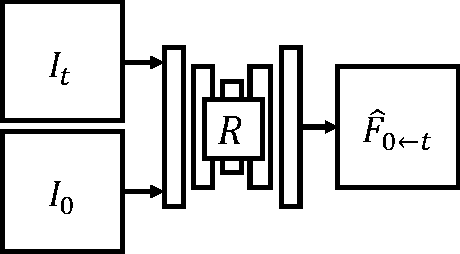
\includegraphics[width=\textwidth]{images/registration_test_start.pdf}\vspace{2.5mm}
        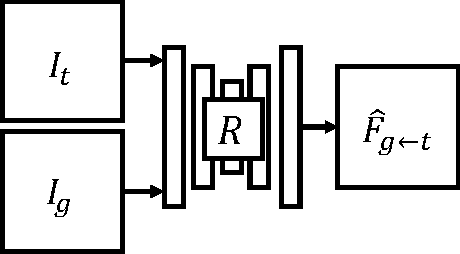
\includegraphics[width=\textwidth]{images/registration_test_goal.pdf}
        \caption{\small{Testing usage.}}
    \end{subfigure}
    \quad \quad
    \begin{subfigure}[b]{0.55\textwidth}
        \centering
        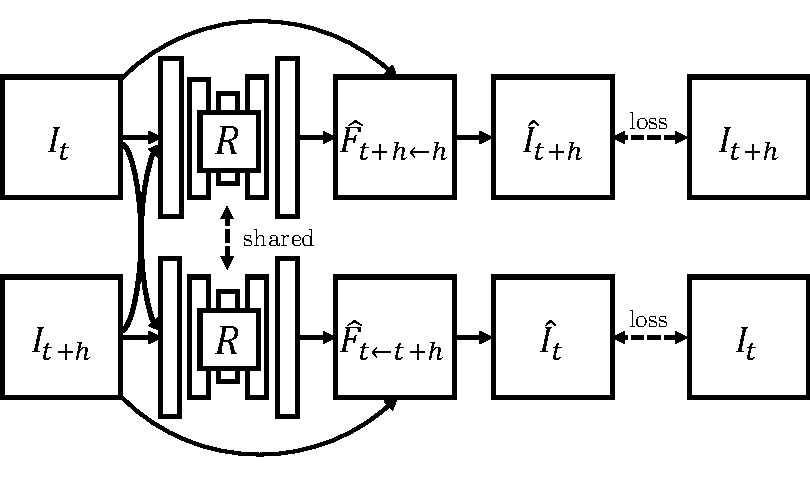
\includegraphics[width=\textwidth,trim={0 3mm 0 3mm},clip]{images/registration_train.pdf}
        \caption{\small{Training usage.}}
        \label{fig:discrete}
    \end{subfigure}
    \vspace{-1mm}
    \caption{\small{(a) At test time the registration network registers the current image $I_t$ to the start image $I_0$ (top) and goal image $I_g$ (bottom), inferring the flow-fields $\hat{F}_{0 \leftarrow t}$ and $\hat{F}_{g \leftarrow t}$. (b) The registration network is trained by warping images from randomly selected timesteps along a trajectory to each other.
    }}
    \label{fig:registration_arch}
\end{figure}

\begin{figure}
    \centering
    \vspace{-0.1in}
    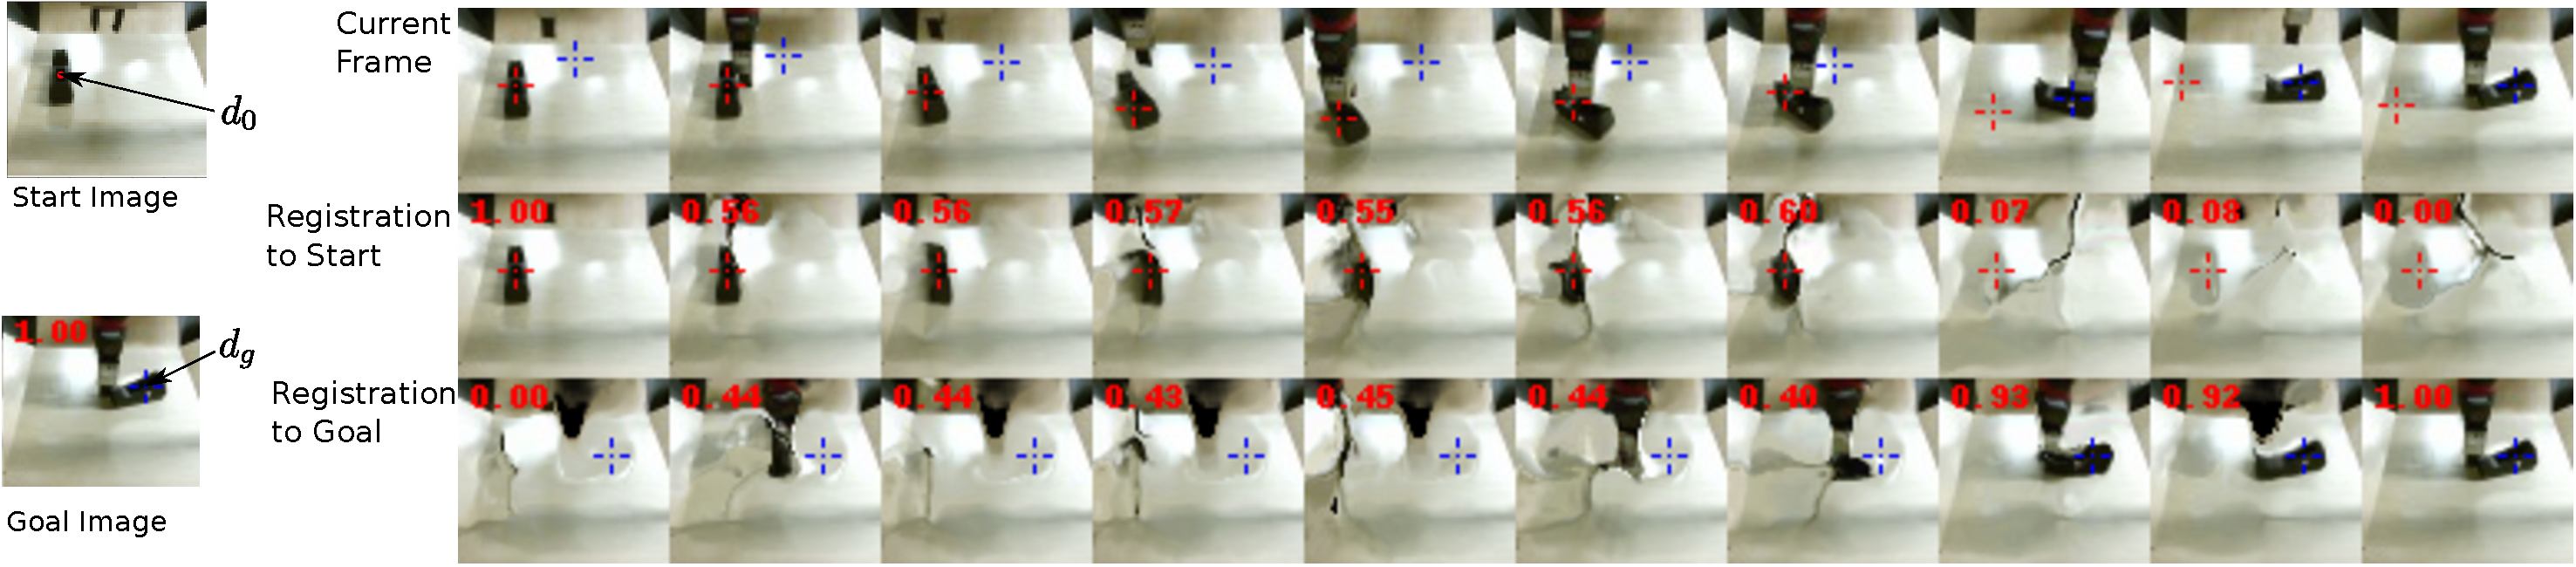
\includegraphics[width=1\textwidth]{images/registration_overtime.pdf}
    \caption{\small{Outputs of registration network. The first row shows images from a trajectory executed by the robot, the second shows each image warped to the initial image via registration, and the third shows the same for the goal image. A successful registration in this visualization would result in images that closely resemble the start (or goal). In these images, the locations where the designated pixel of the start image $d_0$ and the goal image $d_g$ are found is marked with red and blue crosses, respectively. It can be seen that, for the registration to the start image (red cross) the object is tracked for the first 7 frames, while the registration to the goal image (blue cross) succeeds for the last 3 time steps. The numbers in red indicate the trade off factors $\lambda$ between the views and are used as weighting factors for the planning cost.}}
    \label{fig:tracking_overtime}
    \vspace{-0.2in}
\end{figure}

\autoref{fig:tracking_overtime} visualizes the tracking results during a pushing task. On the left we show the start image and goal image provided by the user at the beginning of the trajectory. The first row shows the video, with the estimated location of $d_0$ marked in red and the estimated location of $d_g$ marked in blue. In this example, registration succeeds with respect to the first image succeeds for the first 7 steps but fails after that. However registration with respect to the goal image succeeds for the last 3 steps. Thus, there is enough information at each time step to determine the cost, which we discuss in detail in the next section.

%%SL.06.12: Something to keep in mind here: When describing a learned model, often a good recipe is to first explain the model itself (which is what you're doing here), and then explain how that model is trained. It's important to stick to good abstraction. If the model implementation (i.e., the neural net) is complicated, it can help to first explain it abstractly, then explain the objective, and only then explain how it is instantiated in a neural network. Perhaps this organization can be adopted in this section.



%SL.06.12: I think we need a separate paragraph that discusses two views... this paragraph seems to mix together two different things

%%SL.06.12: for top-level organization, we should have separate subsections for registration and for control. Maybe a reasonable top-level organization I might suggest is:
% 3 Preliminaries
% 4 Overview (summarize how the method works and say what the parts are, so the sections that follow don't come as a surprise)
% 5 Retrying with Registration
% 5.1 Self-Supervised Registration of Goal and Source Images <- this would have \paragraphs for algorithm, training/objective, and model
% 5.2 Deriving Planning Costs from Self-Supervised Registration <- can mention designated pixels here
% 6 Task Setup and Implementation <- all the stuff about how the task is set up, action space, etc
% of course, other organizations are possible, but maybe this gives a hint for how to get started





\vspace{-0.1cm}
\section{Planning Costs}
\vspace{-0.2cm}
As shown in the previous section, registration can fail when distances between objects in the images are large. Here we propose a mechanism that estimates which image is registered correctly, allowing us to utilize only the successful registration for evaluating the planning cost.
When registering to both start and goal-image or when using more than one view, every pair of designated pixel and goal pixel defines a cost function (the expected distance to to the goal). As the robot approaches the goal, the difference to the initial image increases, making it increasingly harder to register. However, the difference to the goal image (hopefully) decreases, making it easier to register.
We exploit this to compute accurate costs for all stages of the task by using a weighting factor that gives a high weight to the designated pixels $\hat{d}_{i,t}$ that are successfully tracked and a low (ideally zero) weight to the designated pixels where the registration is poor. We propose to use the photometric distance (we found that the norm in RGB space works well) between the true frame and the warped frame as an estimate for \emph{local} registration success. A low photometric error indicates that the registration network predicted a flow vector leading to a pixel with a similar color, thus indicating warping success. However this does not necessarily mean that the flow vector points to the correct location. For example, there could be several objects with the same color and the network could simply point to the wrong object. Letting $I_i(d_i)$ denote the pixel value in image $I_i$ for position $d_i$, and $\hat{I}_i(d_i)$ denote the corresponding pixel in the image warped by the registration function (i.e., $\hat{I}_i = \hat{F}_{i \leftarrow t} \diamond I_t$, where $I_t$ is the current image), we can define the general weight factors $\lambda_i$ as
\begin{align}
\lambda_i =  \frac{||I_i(d_i) - \hat{I_i}(d_i)||_2^{-1}}{\sum^N_j ||I_j(d_j) - \hat{I}_j(d_j)||^{-1}_2}.
\label{eqn:cost_avg}
\end{align}
In the case of the single view model and a single designated pixel, the index $i$ iterates over the start and goal image (and $N=2$), in the case of multi-view models or multiple designated pixels the index also loops over the views and indices of the designated pixels. 
The MPC cost is then computed as the average of the costs $c_i$ weighted by $\lambda_i$, where each $c_i$ is the expected distance (see \autoref{eq:cost}) between the predicted pixel positions starting from the registered point $\hat{d}_{i,t}$ and the goal point $d_{g,i}$, where the registered point is found by $\hat{d}_{i,t} = d_i + \hat{F}_{i \leftarrow t}(d_i)$ (analogous to \autoref{eqn:warped_pos}). Finally the cost used for planning is $c = \sum_i \lambda_i c_i$.


\subsection{Training procedure}
\label{subsec:training}
For registration we use a deep convolutional neural network $R$ which takes in a pair of images and finds correspondences by warping one image to the other. The network is trained on the same data as the video-prediction model, but it does not share parameters with it.\footnote{in principle sharing parameters with the video-prediction model might be beneficial, however this is left for future work} Our approach is similar to the optic flow method proposed by \citet{meister2017unflow}. However, unlike this prior work, our method computes registrations for frames that might be many time steps apart, and the goal is not to extract optic flow, but rather to determine correspondences between potentially distant images. For training, two images are sampled at random times steps $t$ and $t+h$ along the trajectory and the images are warped to each other in both directions. 
\begin{align}
     \hat{I}_{t} = \hat{F}_{t \leftarrow t +h} \diamond  I_{t+h} &&
     \hat{I}_{t+h} = \hat{F}_{t+h \leftarrow t} \diamond  I_{t}
\end{align}
The network, which outputs $\hat{F}_{t \leftarrow t +h}$ and $\hat{F}_{t+h \leftarrow t}$ (see Figure~\ref{fig:registration_arch}), is trained to minimize the photometric distance between $\hat{I}_t$ and $I_t$ and $\hat{I}_{t+h}$ and $I_{t+h}$, in addition to a smoothness regularizer that penalizes abrupt changes in the outputted flow-field. The details of this loss function follow prior work \cite{meister2017unflow}. We found that gradually increasing the temporal distance $h$ between the images during training yielded better final accuracy, as it creates a learning curriculum. The temporal distance is linearly increased from 1 step to 8 steps at 20k SGD steps. In total 60k iterations were taken.

The network $R$ is implemented as a fully convolutional network taking in two images stacked together along the channel dimension. We use three convolutional layers each followed by a bilinear downsampling operation. This is passed into three layers of convolution each followed by a bilinear upsampling operation (all convolutions use stride 1). By using bilinear sampling for increasing or decreasing image sizes we avoid artifacts that are caused by strided convolutions and deconvolutions.

\section{Scaling up Visual Model-Predictive Control}
\paragraph{Extension to multiple cameras.}
Prior has considered visual MPC with a single camera~\cite{foresight,sna}, where objects are manipulated on a plane. To define goals in 3D, we extend visual MPC to include multiple camera views (with two cameras in our prototype). Since tasks are defined in terms of pixel motion in 2D image space, the combination of multiple 2D tasks with cameras oriented appropriately defines a 3D task. In our experiments, we show that we can define 3D manipulation tasks (such as lifting an object from the table) that would be ambiguous using only a single camera view. The registration method described in the previous section is used separately per view to allow for dynamic retrying to solve temporally extended tasks. The planning costs from each view are combined using weighted averaging where the weights are provided by the registration network (see equation \ref{eqn:cost_avg}). 

\vspace{-0.1in}
\paragraph{Combined prehensile and non-prehensile manipulation.}
In prior work on video-prediction based robotic manipulation \cite{sna, foresight} the capabilities that emerged out of self-supervised learned were generally restricted to pushing and dragging objects. To enable more complex and temporally extended tasks, we also explore how visual MPC can enable behaviors that include picking and lifting objects for rearrangement. One of the main challenges with this is that random exploration is unlikely to pick up objects a sufficiently large fraction of the time to allow the model to learn grasping skills. To alleviate this challenge, we provide a simple ``reflex'' to the robot during data collection, where the gripper automatically closes when the height of the wrist above the table is lower than a small threshold. This reflex is inspired by the palmar reflex observed in infants~\cite{grasping_fetal}. With this primitive, about 20\% of training trajectories included some sort of grasp on an object. It is worth noting that, other than this reflex, no grasping-specific engineering was applied to the policy, and the video prediction model still needed to learn to predict the raw image frames of these grasps to take advantage of picking skills. In our experiments, we evaluate our method using data obtained both with and without the grasping reflex, evaluating both purely non-prehensile and combined prehensile and non-prehensile manipulation.

%An important advantage of the proposed grasping primitive is that it allows for holding an object continuously for extended periods of time. This also greatly reduces the search space for good successful grasping actions. Without this primitive finding an action sequence for picking up and object and bringing it to a desired location would require sampling actions where the gripper does not open even once while the object is being lifted. Sampling such actions sequences from simple hand-picked distributions (such as a Gaussian) is very unlikely and would therefore dramatically increases the number of samples necessary. We verified in simulation (using CEM and sampling trajectories from the phyiscs engine) that finding action sequences for solving simple pick-up tasks requires around 10 times less samples using the proposed grasping primitive.

%15.000 trajectories were collected using random endeffector motions and the described grasping primitive. We found that our video-prediction is able to learn a joint model for the physics of prehensile and non-prehensile manipulation as shown in \autoref{}. 







\vspace{-0.1cm}
\section{Experiments}
\vspace{-0.2cm}

\begin{wrapfigure}{r}{.35\columnwidth}
\vspace{-0.3in}
\centering
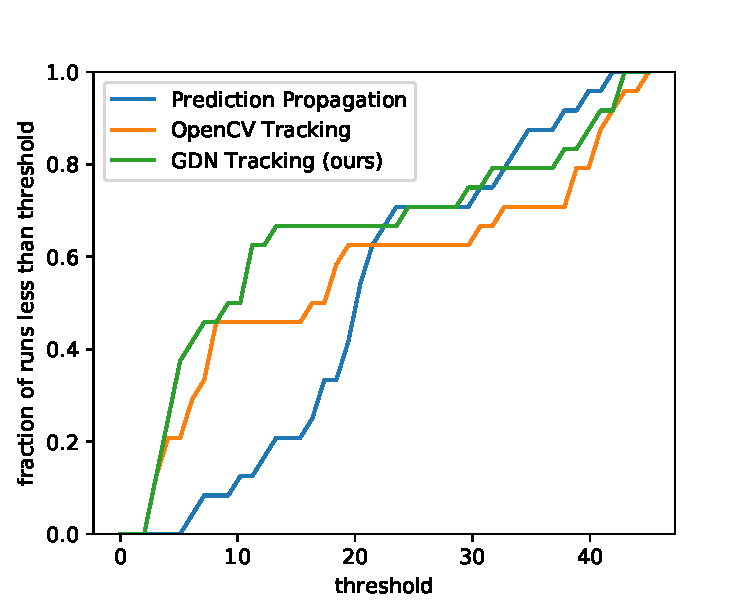
\includegraphics[width=0.35\columnwidth]{images/pushing_score_cdf_robot.pdf}
\caption{\small{Real-world benchmark for pushing with 20 different tasks evaluated on unseen objects. Fraction of runs where final distance (in pixel units of 48x64 image) is lower than threshold. Our method shows a clear gain over OpenCV tracking and predictor propagation.}}
\label{fig:push_bench}
\vspace{-0.3in}
\end{wrapfigure}

Our experimental evaluation, conducted using two Rethink Sawyer robotic manipulators, evaluate the ability of our method to learn both prehensile and non-prehensile object relocation tasks entirely through autonomously collected data and self-supervision. In particular, we aim to answer the following questions: (1) How does our MPC approach with self-supervised goal image registration compare to alternative cost functions, such as off-the-shelf tracking, forward prediction via flow-based models, and pixel difference costs? (2) When the robot can continuously retry a task with goal image registration, how much is the success rate for object relocation tasks improved? (3) Can we learn predictive models that enable both non-prehensile and prehensile object manipulation? We also present additional experimental comparisons in a simulated environment.
Videos and visualizations can be found on this webpage: \url{https://sites.google.com/view/robustness-via-retrying}.

\subsection{Real-World Experiments}

To train both our prediction and registration models, we collected 20,000 trajectories of pushing motions and 15,000 trajectories with gripper control, where the robot was allowed to randomly move and pick up objects. The data collection process is fully autonomous, requiring human intervention only to replace and change out the objects in front of the robot.
%%SL.06.15: would be nice to have a picture of data collection maybe?
The action space consisted of Cartesian movements along the $x$, $y$, and $z$ axes, and changes in azimuthal orientation of the gripper. For evaluation, we selected novel objects that were never seen during training. The evaluation tasks required the robot to move objects in its environment from a starting state to a goal configuration, and performance was evaluated by measuring the distance between the final object position and goal position. In all experiments, the maximum episode length was 50 time steps.

\vspace{-0.1in}
\paragraph{Pushing with retrying.}
\begin{figure}
    \centering
    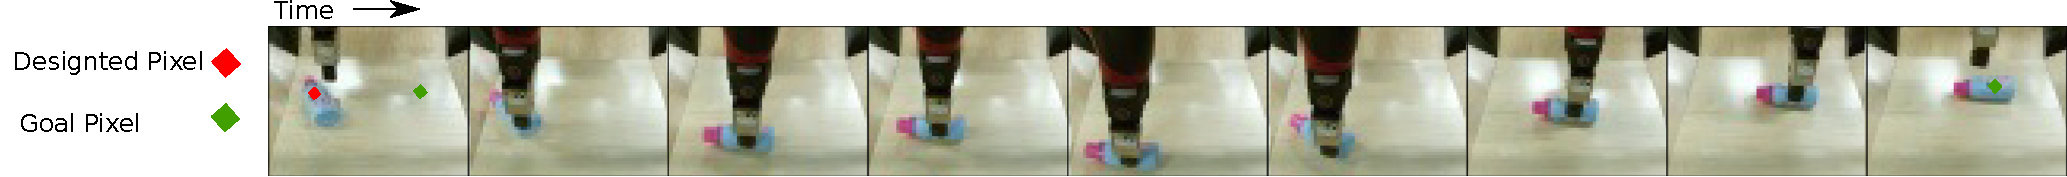
\includegraphics[width=1.0\textwidth]{images/push_correction.pdf}
    \caption{\small{Applying our method to a pushing task. In the first 3 time instants the object behaves unexpectedly, moving down. The tracking then allows the robot to retry, allowing it to eventually bring the object to the goal.}}
    \label{fig:push_retry}
\end{figure}

\begin{figure}
\vspace{-0.1in}
    \centering
    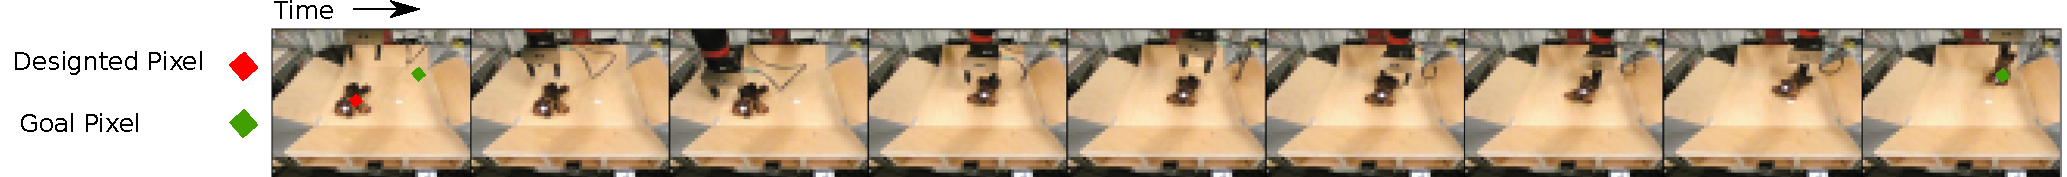
\includegraphics[width=1.0\textwidth]{images/pick_place_plush.pdf}
    \caption{\small{Retrying behaviour of our method combining prehensile and non-prehensile manipulation. In the first 4 time instants shown the agent pushes the object. It then loses the object, and decides to grasp it pulling it all the way to the goal. Retrying is enabled by applying the learned registration to both camera views (here we only show the front view).}}
    \label{fig:discrete}
    \vspace{-0.2in}
\end{figure}

In the first experiment, we aim to evaluate the performance of different visual MPC cost functions, including our proposed self-supervised registration cost. For this experiment, we disable the gripper control, which requires the robot to push objects to the target. We evaluate 20 different pushing tasks that require pushing an object to a target position. For comparisons, we include a baseline where the object is tracked using the ``multiple instance learning tracker'' MIL \cite{babenko2009visual} in OpenCV. Note that our method does not have any prior knowledge of objects -- it is only provided with the position of one designed pixel in the initial and goal images, and must use the learned model to infer that this pixel belongs to an object that can be moved by the robot. We also compare to the visual MPC method proposed by \citet{sna},
%%SL.06.15: fill in citation
which does not track the object explicitly, but relies on the flow-based video prediction model to keep track of the designated pixel, which we call ``predictor propagation.'' We also tested a method where the visual MPC cost is calculated by directly evaluating the error between the predicted image and goal image, but we found that this approach was unable to make meaningful progress in moving the object to the target. Instead it resulted in a policy that always moves the arm to the position indicted in the target image, as the arm accounts for the majority of the movable pixel mass in the image. This can be interpreted as undesirable local minimum which is not present in tracking based cost we propose.

\autoref{fig:push_bench} illustrates that our approach not only outperforms prior work \cite{sna}, but also outperforms the hand-designed object tracker \cite{babenko2009visual}. This is due to the fact that using our learned registration the agent is more frequently able to successfully recovering from situations where the object behaved differently than predicted the model predicted (see \autoref{fig:push_retry}).
%%SL.06.15: fill in discussion about what it does

\vspace{-0.1in}
\paragraph{Combined prehensile and non-prehensile manipulation.}

\begin{wrapfigure}{r}{.35\columnwidth}
\vspace{-0.3in}
\centering
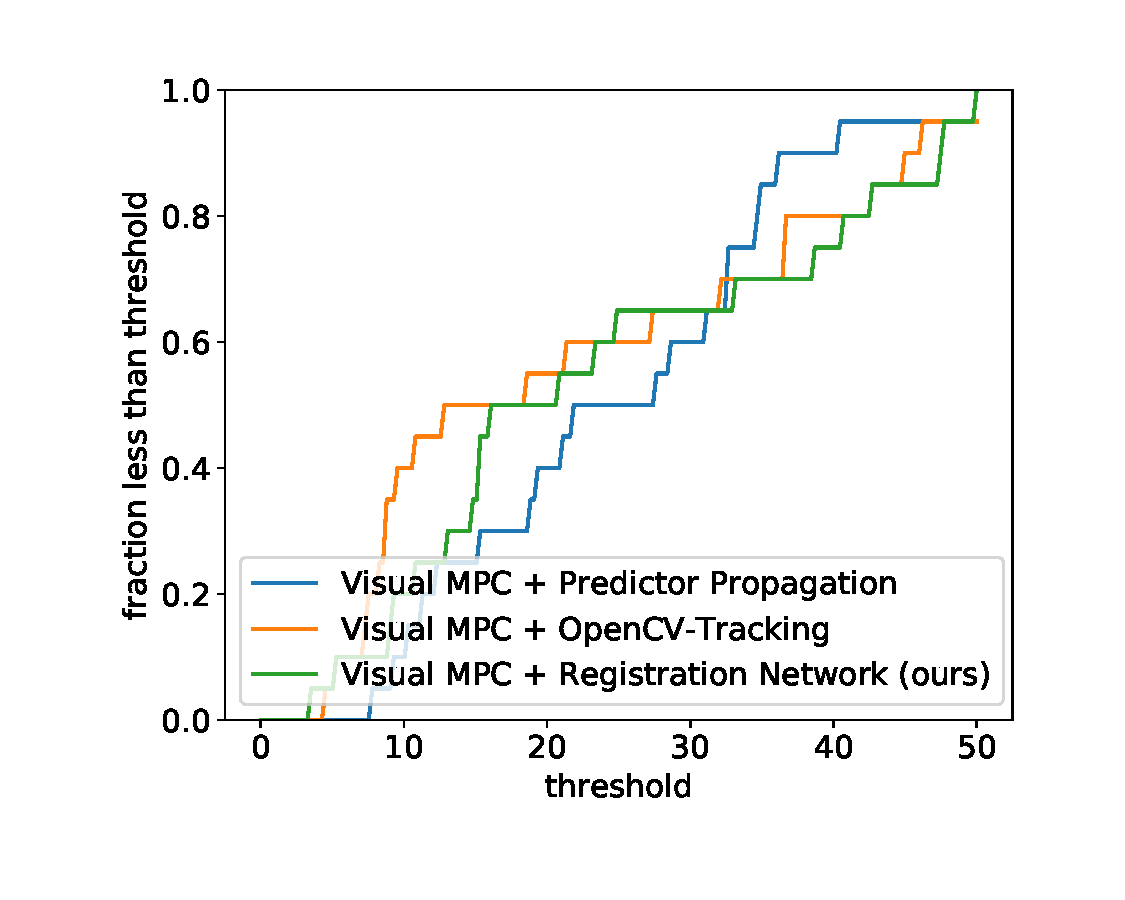
\includegraphics[width=0.35\columnwidth]{images/grasping_score_cdf.pdf}
\caption{\small{On the real-world grasping benchmark our method is on par with OpenCV tracking.}}
\label{fig:grasp_bench}
\vspace{-0.3in}
\end{wrapfigure}


In the setting where the gripper is enabled it is part of the task to decide whether to solve a task by prehensile or non-prehensile manipulation. Similarly to the pushing setting we perform a benchmark where we define a set of 20 object relocation tasks and measure the final distance between the object and the target at the end of the episode. Interestingly we observe that in the majority of the cases the agent decides to grasp the object, as can be seen in the supplementary video. \autoref{fig:grasp_bench} shows that the performance of our method is comparable with the performance of OpenCV tracking.




\section{Discussion}

In both \cite{hermans2013learning,salganicoff1993vision} pushing of unknown objects is learned from interaction data between the robot and objects. However the models employed in these works rely on hand-engineered input features (e.g. in the form of the approach angle to the object \cite{salganicoff1993vision} or a set of points on the silhouette of an object \cite{hermans2013learning}) which can make it hard to scale to complex real-world scenarios where for example objects can be partially occluded or cluttered. 
It as been shown in \cite{goldfeder2009data} and others that grasps on unseen objects can be found by matching the sensed 3D geometry to a database of precomputed object-grasp pairs. One downside to this approach is that physics are generally ignored in this scheme. For example information about mass and friction properties which can be estimated from visual clues (but not from geometry alone) cannot be leveraged. In \cite{mahler2017dex} large databases of 3D meshes are used to label synthetic depth images with an analytic physics based grasp quality metric. This approach has the downside of relying on a suitable metric which is not available for other manipulation tasks (such as pushing) in general.
Furthermore most prior approaches are not capable of selecting whether a grasping or pushing (or dragging) strategy is better suited to solve the given task and also do not exhibit a "retrying" behavior for recovering from failure.
Video-prediction based manipulation is more general than many existing methods for robotic manipulation such as grasping specific \cite{lenz2015deep, goldfeder2009data, zeng2017robotic} or pushing specific works \cite{hermans2013learning, salganicoff1993vision} because it does not require any human intervention at training time (i.e. human labels), large databases of 3D objects meshes and does not make any assumptions about object boundaries or the dimensionality of the state space.

Our method uses a video prediction model to predict future frames from autonomously gathered exploration data, and uses this same data to train a registration model that can be used to evaluate the distance to the goal for the predicted frames. We demonstrate that using a cost function derived from this distance substantially improves performance on temporally extended tasks. We further show that, by including a simple grasping ``reflex'' inspired by the palmar reflex in infants, we can effectively learn both non-prehensile and prehensile object relocation skills, allowing the robot to plan to pick up and move objects when necessary. Our experiments show a large improvement in success rates compared to a prior visual MPC method~\cite{sna}.


%===============================================================================

% The maximum paper length is 8 pages excluding references and acknowledgements, and 10 pages including references and acknowledgements

%\clearpage
% The acknowledgments are automatically included only in the final version of the paper.
%\acknowledgments{If a paper is accepted, the final camera-ready version will (and probably should) include acknowledgments. All acknowledgments go at the end of the paper, including thanks to reviewers who gave useful comments, to colleagues who contributed to the ideas, and to funding agencies and corporate sponsors that provided financial support.}

%===============================================================================

% no \bibliographystyle is required, since the corl style is automatically used.
\bibliography{bib}  % .bib


\newpage
\appendix

{\footnotesize
\part*{Appendix}


\subsection*{Simulated Experiments}


\begin{wrapfigure}{r}{.34\columnwidth}
	\centering
	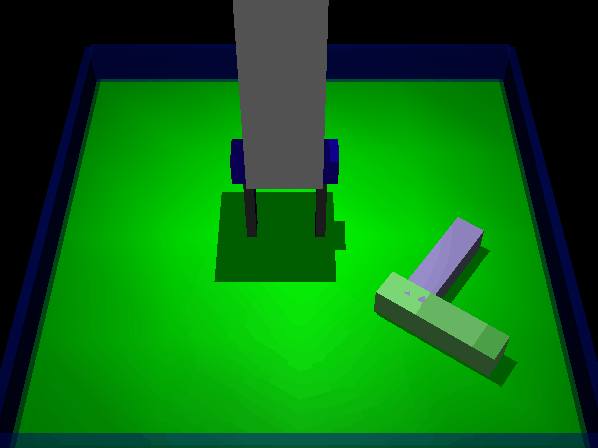
\includegraphics[width=0.3\columnwidth]{images/simulator.png}
	\caption{\small{Block pushing simulator}}
	\label{fig:sim}
\end{wrapfigure}

In order to provide a more controlled comparison, we also set up a realistic simulation environment using MuJoCo \cite{todorov2012mujoco}, which includes a robotic manipulator controlled via Cartesian position control, similar to our real world setup, pushing randomly-generated L-shaped objects with random colors (see details in supplementary materials). 
We trained the same video prediction model in this environment, and set up 50 evaluation tasks where blocks must be pushed to target locations with maximum episode lengths of 120 steps. 
\begin{wrapfigure}{r}{.4\columnwidth}
	\centering
	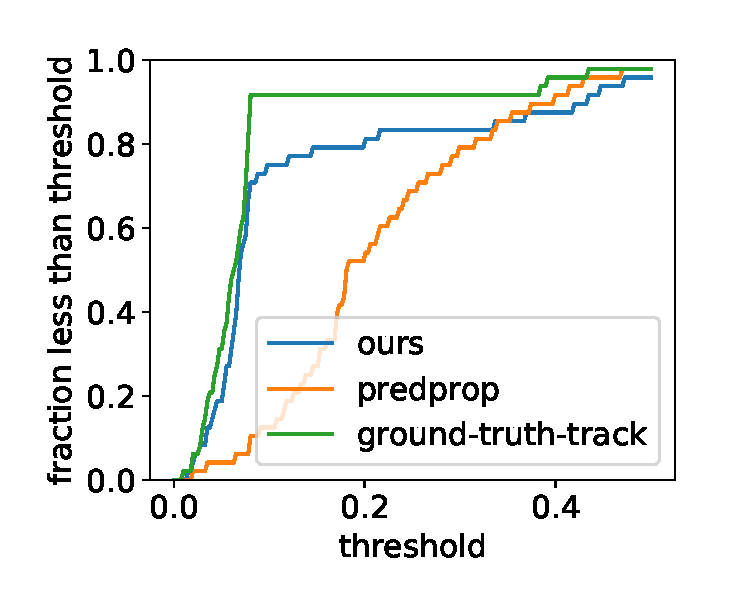
\includegraphics[width=0.4\columnwidth]{images/2obj_scores_ours-predprop-ground-truth-track.pdf}
	\caption{\small{Simulated evaluation. Fraction of trajectories with final object distance lower than threshold (higher is better).}}
	\label{fig:sim_bench}
\end{wrapfigure} 


We  compare our proposed registration-based method, ``predictor propagation,'' and ground-truth registration obtained from the simulator, which provides an oracle upper bound on registration performance. \autoref{fig:sim_bench} shows the results of this simulated evaluation, where the x-axis shows different distance thresholds, and the y-axis shows the fraction of evaluation scenarios where each method pushed the object within that threshold. We can see that, for thresholds around 0.1, our method drastically outperforms predictor propagation (i.e., prior work~\cite{sna}), and has a relatively modest gap in performance against ground-truth tracking. This indicates that our registration method is highly effective in guiding visual MPC, despite being entirely self-supervised.

In our simulated experiments, we use end-effector position control with the arm illustrated in Figure~\ref{fig:sim}. In this environment, the video prediction model was trained with using 60,000 training trajectories.

\section*{Planner Implementation Details}

We use the cross-entropy method \cite{cem-rk-13} to optimize the action sequence with respect to the cost function. At the first iteration 400 samples and at later iterations 200 samples are taken and  a Gaussian is fitted to the best $5\%$ of the samples. We use 3 CEM iterations. The length of the prediction horizon is 15, to reduce the search space we use an action repeat of 3, so that only a sequence of 5 independent actions needs to be optimized. Since the action space is 4 (x,y,z,rotation) a total of 20 variables are optimized.

\section*{Improvements to online optimization procedure}
In the visual MPC setting the action sequences found by the optimizer can be very different between execution times steps (not to be confused with prediction time steps). For example at one time step the optimizer might find a pushing action leading towards the goal and in the next time step it determines a grasping action to the optimal to reach the goal. Naive replanning at every time step can result in alternating between a pushing attempt and a grasping attempt indefinitely causing the agent to get stuck and not making any progress towards to goal. 

We show that we can resolve this problem by modifying the sampling distribution of the first iteration of CEM so that the optimizer commits to the plan found in the previous time step. In prior work \cite{sna} the sampling distribution at first iteration of CEM is chosen to be a Gaussian with diagonal covariance matrix and zero mean. We instead use the best action sequence found in the optimization of the previous time step as the mean. Since this action sequence is optimized for the previous time step we only use the values $a_{1:T}$ and omit the first action, where $T$ is the prediction horizon. To sample actions close to the action sequence from the previous time step we reduce the entries of the diagonal covariance matrix for the first $T-1$ time steps. It is crucial that the last entry of the covariance matrix at the end of the horizon is not reduced otherwise no exploration could happen for the last time step causing poor performance at later time steps.
}

\end{document}
